% This manuscript was migrated from the old IEEE LaTeX source to the
% MICCAI 2025 LNCS conference template. Content is preserved; only the
% document shell and formatting packages were adapted.
\documentclass[runningheads]{llncs}

\usepackage[T1]{fontenc}
\usepackage{graphicx,verbatim}
\usepackage{amsmath}
\usepackage{amssymb}
\usepackage{booktabs}
\usepackage{array}
\usepackage{bm}
\usepackage{url}
\usepackage[hidelinks]{hyperref}

% ---- Convenience macros preserved from the old source ----
\newcommand{\iou}{\mathrm{IoU}}
\newcommand{\monitor}{TCSR-Monitor}
\newcommand{\unet}{U-Net}

\begin{document}

\title{Generalization-Aware Safety Monitoring for Surgical\\
Segmentation Failures under Acquisition Degradation}
\titlerunning{Monitoring Surgical Segmentation Failures}

\author{Anonymized Authors}
\authorrunning{Anonymized Author et al.}
\institute{Anonymized Affiliations \\
    \email{email@anonymized.com}}

\maketitle

\begin{abstract}
Surgical segmentation networks can fail silently under acquisition degradation:
the mask is wrong, yet the network remains confident. We present
\monitor{}, a generalization-aware safety-monitoring framework that maps
$22$ observable confidence, shape, temporal, and image-quality features from a
frozen segmenter to a failure-risk score. The contribution is not only a
detector, but a validity protocol for asking whether learned alarms remain
credible under distribution shift. On EndoVis~2017 instrument segmentation,
\monitor{} attains AUROC $0.814$ on unseen corruption types under
leave-one-corruption-out (LOCO) evaluation, winning $26$ of $30$ held-out
conditions against entropy. A circularity-control experiment shows that the
monitor predicts segmentation failure rather than merely detecting corruption
(within-corrupted AUROC $0.946$, $[0.943,0.949]$). A learned confidence-only
control is strong, but the full feature set improves LOCO AUROC/AUPRC at
$\tau=0.75$ from $0.912/0.888$ to $0.920/0.903$. Finally, Mondrian
group-conditional conformal calibration restores near-target per-severity
miss-rate at $\alpha=0.10$ (severity-1 miss $50.5\%\rightarrow9.3\%$), while
making the increased frame-level alarm burden explicit. Zero-shot transfer to
SAM2-Tiny reaches AUROC $0.930$ $[0.912,0.945]$, supporting feature
portability but also showing that entropy remains strong when failures are
already expressed as uncertainty.

\keywords{Surgical segmentation \and Failure monitoring \and Conformal prediction}
\end{abstract}

\section{Introduction}

Deep segmentation networks are increasingly used to parse endoscopic video
into instrument and anatomy masks~\cite{ref:shvets,ref:allan}, but deployed
surgical video contains smoke, defocus, illumination change, compression, and
motion blur that are under-represented in curated benchmarks. These acquisition
shifts can produce \emph{silent failures}: masks with low intersection-over-union
(IoU) despite high output confidence. Such failures are safety-critical because
standard confidence monitors---max-softmax~\cite{ref:hendrycks}, predictive
entropy~\cite{ref:malinin}, and calibration-based scores~\cite{ref:guo}---measure
uncertainty. If a wrong mask is also confident, uncertainty is low by
construction.

\monitor{} addresses this gap by learning observable failure patterns rather
than directly reading uncertainty. It wraps a frozen segmenter, extracts
confidence, morphology, temporal-consistency, and image-quality features, and
predicts whether the segmenter has failed without accessing ground truth at
deployment. A learned monitor, however, is useful only if it survives three
validity tests: it must generalize beyond seen degradations, predict failure
rather than corruption presence, and support calibrated alarm thresholds across
degradation severity. This paper is organized around those tests.

\noindent\textbf{Contributions.}
\begin{enumerate}
\item a lightweight failure monitor for frozen surgical segmenters using
observable confidence, shape, temporal, and image-quality features;
\item a protocol-qualified generalization hierarchy showing AUROC $0.814$ on
unseen corruption types under LOCO evaluation;
\item a circularity control showing that the monitor predicts failure rather
than corruption presence (within-corrupted AUROC $0.946$);
\item Mondrian conformal calibration that reduces severity-1 miss-rate from
$50.5\%$ to $9.3\%$ at $\alpha=0.10$, while exposing the false-alarm cost;
\item supporting controls, reported in the supplement, that bound the claim
against confidence-only, learner, temporal-order, sequence-held-out, and SAM2
transfer alternatives.
\end{enumerate}

The intended use is not to replace segmentation, but to add a fast, external
watchdog for cases in which the segmenter remains confident while its mask
quality collapses. This distinction also determines the evaluation: a monitor
that performs well only after seeing the same corruption operators during
training is less useful than one whose failure score transfers across unseen
degradation types.

%%%%%%%%%%%%%%%%%%%%%%%%%%%%%%%%%%%%%%%%%%%%%%%%%%%%%%%%%%%%%%%%%%%%%%%%%%%%%%%%
\section{Related Work}

Instrument segmentation has advanced through \unet{} variants~\cite{ref:ronneberger},
transformers~\cite{ref:dong}, and foundation models such as SAM/SAM2
~\cite{ref:kirillov,ref:ravi}. Robustness benchmarks expose sensitivity to
common or surgical corruptions~\cite{ref:hendrycks_c,ref:segstrong,ref:michieli},
but they primarily evaluate the segmenter itself. Our focus is deployment-time
monitoring after a mask has already been produced.

Confidence scores, entropy, calibration, test-time ensembles, and feature-space
OOD scores are common post-hoc reliability signals
~\cite{ref:hendrycks,ref:malinin,ref:guo,ref:lakshmi,ref:lee}. In medical
segmentation, however, uncertainty can be calibrated in aggregate while still
failing on individual cases~\cite{ref:jungo}, and networks may remain
overconfident on wrong masks~\cite{ref:mehrtash}. Learned failure prediction
therefore provides a complementary route: prior work estimates model confidence
or segment quality from auxiliary signals~\cite{ref:corbiere,ref:granese,ref:rottmann,ref:fsnet}.
We differ by centering surgical acquisition degradation, held-out corruption
protocols, and a circularity control that separates failure prediction from
corruption detection. Our alarm layer relates to selective prediction
~\cite{ref:geifman,ref:selectivenet} and conformal risk control
~\cite{ref:vovk,ref:angelo_intro,ref:crc}; group-conditional Mondrian
calibration~\cite{ref:mondrian} is especially natural when degradation severity
defines safety-relevant groups.

%%%%%%%%%%%%%%%%%%%%%%%%%%%%%%%%%%%%%%%%%%%%%%%%%%%%%%%%%%%%%%%%%%%%%%%%%%%%%%%%
\section{Method}

\monitor{} wraps a frozen segmenter $f_\theta$ without changing its weights.
For each frame $I_t$, the segmenter produces a probability map $p_t$ and mask
$\hat y_t$. A frame is labeled a failure during training/evaluation when
\begin{equation}
\mathrm{fail}(I_t)=\mathbf{1}\!\left[\iou(\hat{y}_t,y_t^\star)<\tau\right],
\qquad \tau \in \{0.5,\,0.75\}.
\label{eq:failure_label}
\end{equation}

\begin{figure}[t]
\centering
\small
\setlength{\tabcolsep}{3pt}
\resizebox{\textwidth}{!}{\fbox{%
\begin{tabular}{>{\centering\arraybackslash}p{0.15\linewidth}
                c
                >{\centering\arraybackslash}p{0.16\linewidth}
                c
                >{\centering\arraybackslash}p{0.17\linewidth}
                c
                >{\centering\arraybackslash}p{0.16\linewidth}
                c
                >{\centering\arraybackslash}p{0.16\linewidth}}
\textbf{Frame} $I_t$ &
$\rightarrow$ &
\textbf{Frozen segmenter} &
$\rightarrow$ &
\textbf{Observable features} &
$\rightarrow$ &
\textbf{Risk score} &
$\rightarrow$ &
\textbf{Alarm}\\
raw image &&
$p_t,\hat y_t$ &&
confidence, shape, temporal, quality &&
$g_\phi(x_t)$ &&
$g_\phi(x_t)>\lambda_g$
\end{tabular}}}
\caption{Overview of \monitor{}. The monitor observes the raw frame and the
segmenter's output, but does not modify the segmenter or use ground truth at
deployment. Calibration converts risk scores into global or group-specific
alarm thresholds.}
\label{fig:pipeline}
\end{figure}

\noindent The monitor extracts $22$ scalar features from $p_t$, $\hat y_t$,
$I_t$, and previous masks: confidence statistics, mask morphology, temporal
consistency, and image-quality measures (brightness, blur, contrast, specular
ratio). Features require only the raw frame and segmenter output, and take
under $0.5$\,ms per frame (median $0.48$\,ms, $p_{95}$ $0.53$\,ms).

The feature design is intentionally restricted to quantities available outside
the segmentation model. Confidence features capture whether the output looks
uncertain; shape features capture implausible mask geometry and fragmentation;
temporal features capture abrupt changes across adjacent video frames; and
image-quality features capture acquisition conditions that can make a confident
mask suspect. This makes the monitor compatible with frozen clinical models
and avoids relying on architecture-specific internal activations.

The failure-risk model $g_\phi(x_t)\in[0,1]$ is an XGBoost classifier
~\cite{ref:xgboost}; learner ablations in the supplement show that the
representation is not unique to XGBoost. Training uses clean out-of-fold
predictions and corrupted training frames, while threshold calibration is held
out from model fitting. At deployment, ground truth is unavailable and an alarm
is raised when $g_\phi(x_t)>\lambda$.

The safety objective is miss-rate control: among failed frames, the fraction
not alarmed should stay below target $\alpha$:
\begin{equation}
\mathrm{miss}(\lambda)=
\frac{\bigl|\{\, i : g_\phi(x_i) \le \lambda,\; \mathrm{fail}(I_i)=1\,\}\bigr|}
     {\bigl|\{\, i : \mathrm{fail}(I_i)=1 \,\}\bigr|}.
\end{equation}
Global split-conformal calibration~\cite{ref:vovk} chooses one threshold
$\lambda$ on a calibration split. Because acquisition severity changes the
failure distribution, we also use Mondrian calibration~\cite{ref:mondrian}:
frames are partitioned into groups $g$ (corruption severity for degraded
frames; blur tertile for clean frames), and each group receives its own
threshold
\begin{equation}
\lambda_g = \sup\!\left\{ \lambda :
\frac{\bigl|\{\, i \in \mathcal{G}_g : g_\phi(x_i) \le \lambda,\; y_i = 1 \,\}\bigr|}
     {\bigl|\{\, i \in \mathcal{G}_g : y_i = 1 \,\}\bigr|} \le \alpha \right\}.
\end{equation}
This equalizes empirical conservatism across groups rather than letting easy
conditions dominate the average.

The thresholds are calibrated after score learning. Thus discrimination
(whether failures rank above correct frames) and safety control (where to set
the alarm threshold) are evaluated separately. This separation is important in
rare-event settings: a high AUROC monitor can still be operationally burdensome
if the threshold required to catch failures creates many frame-level alarms.

%%%%%%%%%%%%%%%%%%%%%%%%%%%%%%%%%%%%%%%%%%%%%%%%%%%%%%%%%%%%%%%%%%%%%%%%%%%%%%%%
\section{Experiments}

\subsection{Setup}

We use EndoVis~2017 Instrument Segmentation~\cite{ref:bodenstedt}: ten robotic
surgical sequences, with sequences $1$--$7$ for train/calibration and
$8$--$10$ for test ($1575/450/825$ frames). The frozen segmenter is a
ResNet34-\unet{} fine-tuned on the training sequences. We apply six corruption
types at five severity levels (Gaussian blur/noise, motion blur, brightness,
contrast, JPEG), yielding $24{,}750$ corrupted test frames. We evaluate
$\tau=0.5$ and $\tau=0.75$; clean-test failure prevalence is $1.7\%$ and
$6.9\%$, respectively. Baselines are Max-Softmax, Entropy, and a Temporal
Heuristic, plus a learned confidence-only monitor in the supplement.

We use four generalization protocols. \emph{Zero-shot} trains the monitor on
clean frames only and tests on all corruptions. \emph{LOCO} trains on five
corruption types and tests on the held-out sixth type; this is the robustness
headline because the test degradation operator is unseen. \emph{Severity
extrapolation} trains on severities $1$--$3$ and tests on severities $4$--$5$.
\emph{In-distribution} trains and tests across all corruption types and is
reported only as an upper bound.

\subsection{Clean Test and Generalization}

On held-out clean test (Table~\ref{tab:main}), \monitor{} improves AUROC over
all audited baselines at both thresholds. AUPRC is prevalence-sensitive:
entropy is stronger at $\tau=0.5$, whereas \monitor{} gives the best audited
AUPRC at $\tau=0.75$.

\begin{table}[t]
\caption{Held-out clean test results (seed~0; $95\%$ CI from $1000$ bootstrap
samples where available). AUPRC should be interpreted relative to the rare
failure prevalence.}
\label{tab:main}
\centering
\footnotesize
\setlength{\tabcolsep}{4pt}
\resizebox{\textwidth}{!}{%
\begin{tabular}{lcccc}
\toprule
Method & $\tau=0.5$ AUROC & $\tau=0.5$ AUPRC & $\tau=0.75$ AUROC & $\tau=0.75$ AUPRC \\
\midrule
\textbf{\monitor{} (ours)} & \textbf{0.877} & 0.468 & \textbf{0.793} & \textbf{0.301} \\
Entropy~\cite{ref:malinin}            & 0.764 & \textbf{0.635} & 0.483 & 0.220 \\
Max-Softmax~\cite{ref:hendrycks}      & 0.536 & 0.087 & 0.509 & 0.085 \\
Temporal Heuristic                    & 0.338 & 0.013 & 0.460 & 0.074 \\
\midrule
Failure prevalence                    & \multicolumn{2}{c}{$1.7\%$ ($14/825$)} & \multicolumn{2}{c}{$6.9\%$ ($57/825$)} \\
\bottomrule
\end{tabular}
}
\end{table}

\begin{figure}[t]
  \centering
  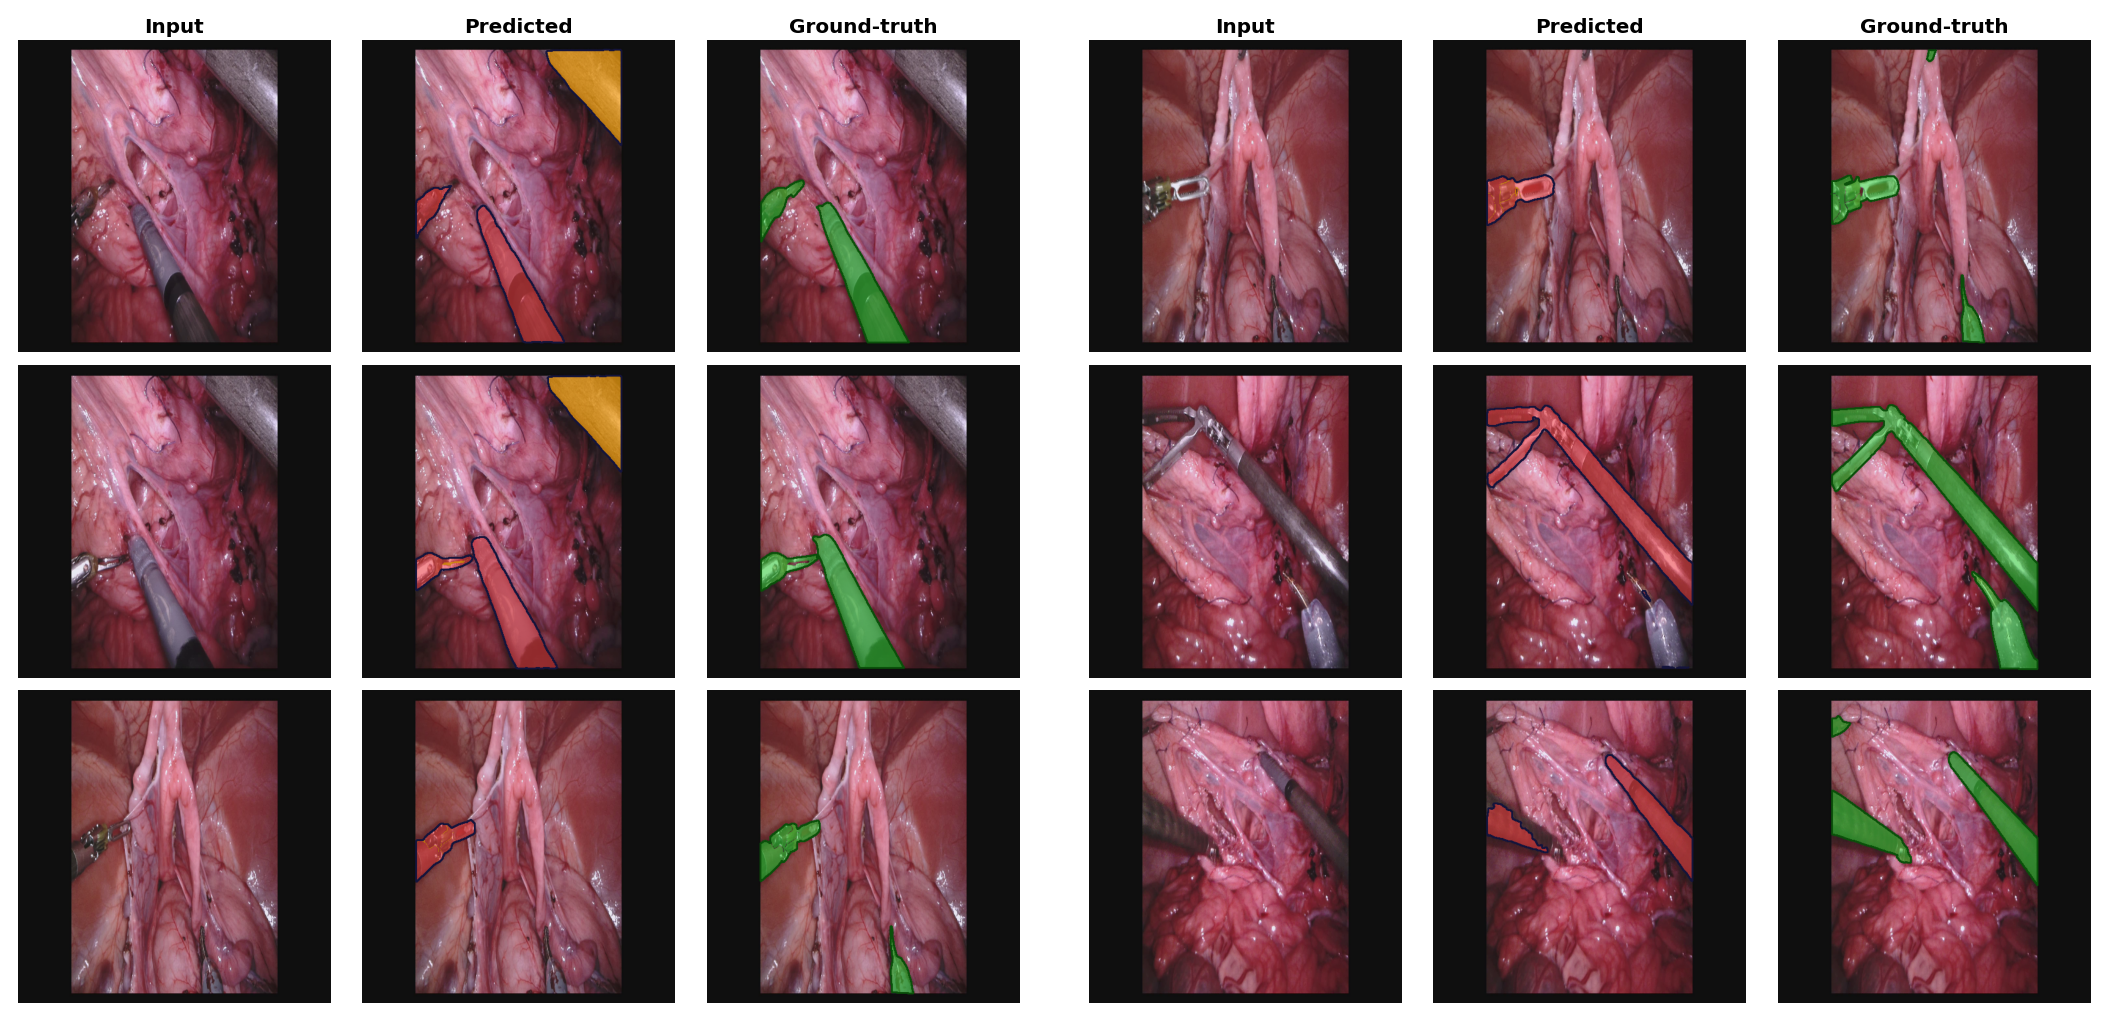
\includegraphics[width=\textwidth]{fig/qual_failures_tau75.png}
  \caption{Qualitative examples of sub-threshold confident failures
  ($0.5 \le \iou < 0.75$). Each triplet shows the input, predicted mask, and
  ground-truth mask. The segmenter produces plausible-looking but incomplete
  or over-extended instruments, illustrating why an external failure monitor is
  needed even when the output appears confident.}
  \label{fig:qualitative}
\end{figure}

\begin{table}[t]
\caption{Generalization hierarchy and LOCO breakdown (AUROC). LOCO is the
robustness headline; in-distribution is an upper bound.}
\label{tab:hierarchy}
\centering
\footnotesize
\setlength{\tabcolsep}{4pt}
\begin{tabular}{lccc}
\toprule
Protocol / held-out type & Monitor & Entropy & Wins \\
\midrule
Zero-shot & 0.753 & 0.465 & 24/30 \\
\textbf{LOCO overall} & \textbf{0.814} & \textbf{0.481} & \textbf{26/30} \\
Severity extrapolation & 0.831 & 0.408 & 8/12 \\
In-distribution upper bound & 0.827 & 0.465 & 26/30 \\
\midrule
Brightness        & 0.801 & 0.331 & 4/5 \\
Contrast          & 0.912 & 0.839 & 3/5 \\
Gaussian blur     & 0.806 & 0.455 & 5/5 \\
Gaussian noise    & 0.811 & 0.319 & 4/5 \\
JPEG compression  & 0.773 & 0.444 & 5/5 \\
Motion blur       & 0.779 & 0.497 & 5/5 \\
\bottomrule
\end{tabular}
\end{table}

LOCO ($0.814$) is the robustness headline because the test corruption type is
absent from training. The small gap to the in-distribution upper bound
($0.827$) argues against simple corruption fingerprinting, and the monitor
beats entropy on all six held-out types.

The clean-test and LOCO results answer different questions. Clean test measures
behavior on nominal deployment-like frames, where failures are rare and AUPRC
is prevalence-sensitive. LOCO stresses whether the learned score captures
transferable failure patterns under acquisition degradation. The combination is
more informative than either setting alone: clean test guards against excessive
alarms on normal video, while LOCO guards against memorizing the training
corruptions.

\subsection{Circularity and Conformal Safety}

To test whether \monitor{} predicts \emph{failure} rather than simply
\emph{corruption}, we evaluate only corrupted test frames and discriminate
correct masks ($\iou\ge0.75$) from failed masks ($\iou<0.75$). Table
~\ref{tab:circularity} shows AUROC $0.946$, while entropy is only $0.594$.
This control is essential because a monitor could otherwise appear successful
by detecting low image quality rather than segmentation failure. Restricting
the evaluation to corrupted frames removes the easy corrupted-versus-clean
shortcut and asks whether the monitor can tell when the segmenter is actually
wrong within degraded video.

\begin{table}[t]
\caption{Circularity control and Mondrian conformal calibration. Left:
within-corrupted AUROC for failure vs.\ correct masks. Right: miss-rate by
severity at $\alpha=0.10$.}
\label{tab:circularity}
\centering
\footnotesize
\begin{tabular}{lccc@{\qquad}lcc}
\toprule
Severity & Monitor & Entropy & FA-correct & Severity & Global miss & Mondrian miss \\
\midrule
1 & 0.807 & 0.484 & 6.5\% & 1 & 50.5\% & 9.3\% \\
2 & 0.844 & 0.391 & 13.3\% & 2 & 22.5\% & 10.1\% \\
3 & 0.802 & 0.260 & 63.7\% & 3 & 9.2\% & 9.9\% \\
4 & 0.861 & 0.366 & 35.8\% & 4 & 6.1\% & 10.0\% \\
5 & 0.825 & 0.478 & 8.9\% & 5 & 5.2\% & 9.9\% \\
\midrule
\textbf{Overall} & \textbf{0.946} & \textbf{0.594} & \textbf{12.6\%} &
\textbf{Overall} & \textbf{10.0\%} & \textbf{9.9\%} \\
\bottomrule
\end{tabular}
\end{table}

Mondrian calibration fixes the safety imbalance hidden by global calibration:
the same overall $10.0\%$ global miss-rate is obtained while missing $50.5\%$
of severity-1 failures. Per-severity thresholds restore near-$10\%$ miss-rate
for all severities, but at a cost: corrupted false-alarm rate increases from
$17.6\%$ to $34.2\%$ overall and from $12.8\%$ to $58.7\%$ at severity~1
(supplement). Thus the claim is safety redistribution, not clinical alarm
readiness.

\subsection{SAM2 Transfer}

We apply the \unet{}-trained monitor to SAM2-Tiny~\cite{ref:ravi} run
zero-shot with oracle bounding-box prompts. SAM2 fails more often than the
fine-tuned \unet{} ($51.2\%$ vs.\ $6.9\%$ at $\tau=0.75$), yet the transferred
monitor reaches AUROC $0.930$ (Table~\ref{tab:transfer}), recovering $93.3\%$
of a SAM2-supervised monitor. Entropy is stronger on SAM2 because these
zero-shot failures appear as high uncertainty; the transfer result supports
feature portability, not universal superiority over uncertainty baselines.

\begin{table}[t]
\caption{Cross-model transfer to SAM2-Tiny.}
\label{tab:transfer}
\centering
\footnotesize
\resizebox{\textwidth}{!}{%
\begin{tabular}{lcc}
\toprule
Condition & $\tau=0.5$ AUROC & $\tau=0.75$ AUROC \\
\midrule
\textbf{\unet{} monitor $\rightarrow$ SAM2} (zero-shot transfer) & \textbf{0.896} $[0.873, 0.915]$ & \textbf{0.930} $[0.912, 0.945]$ \\
Entropy $\rightarrow$ SAM2                                       & 0.984 $[0.975, 0.990]$ & 0.988 $[0.979, 0.994]$ \\
SAM2-specific monitor (upper bound)                             & 0.997 $[0.995, 0.999]$ & 0.997 $[0.994, 0.999]$ \\
Transfer efficiency (transfer / upper bound)                    & 89.8\% & \textbf{93.3\%} \\
\bottomrule
\end{tabular}
}
\end{table}

%%%%%%%%%%%%%%%%%%%%%%%%%%%%%%%%%%%%%%%%%%%%%%%%%%%%%%%%%%%%%%%%%%%%%%%%%%%%%%%%
\section{Discussion}

\monitor{} is best understood as a validation-aware monitoring framework, not
as a claim that one classifier dominates all baselines. The LOCO and
circularity experiments address the two most likely reviewer objections:
corruption fingerprinting and corruption detection. The confidence-only,
learner, temporal, and sequence controls in the supplement narrow the claim:
confidence cues are strong, the full feature set adds modest but positive LOCO
gains, and random forest matches or exceeds XGBoost. The novelty is therefore
the combination of observable features with protocol-qualified validation and
group-conditional safety calibration.

The supplement fills in the main controls behind this interpretation. The
learned confidence-only baseline is deliberately stronger than raw entropy or
max-softmax because it receives the same learner family as the full monitor.
The full feature set improves over it under LOCO, but only modestly, so the
claim is not that confidence is irrelevant. Instead, shape, temporal, and
image-quality features add incremental generalization signal where confident
failures are the target.

The main limitation is scope. All validated discrimination and calibration
results use EndoVis~2017 with synthetic corruptions; real multi-site surgical
video remains future work. A cached CholecSeg8k audit produced failures for
every frame under the current pipeline and therefore could not provide AUROC or
AUPRC external validation. SAM2 uses oracle bounding-box prompts and does not
replace a second fine-tuned surgical-backbone study. Finally, conformal
coverage is empirical rather than certified under temporal dependence, and
frame-level alarm rates are too high for direct clinical use without event
aggregation or workflow suppression.

These limitations narrow the deployment claim. The present evidence supports
\monitor{} as a credible research baseline and validation protocol for
monitoring surgical segmentation under acquisition degradation. It does not yet
establish a clinically deployable alert stream, nor does it prove universal
transfer across hospitals, procedures, or fine-tuned backbone families.

%%%%%%%%%%%%%%%%%%%%%%%%%%%%%%%%%%%%%%%%%%%%%%%%%%%%%%%%%%%%%%%%%%%%%%%%%%%%%%%%
\section{Conclusion}

We presented \monitor{}, a safety-monitoring framework for surgical
segmentation failures under acquisition degradation. By pairing a lightweight
feature-based monitor with LOCO generalization, circularity control, and
Mondrian conformal calibration, the paper provides a credible and bounded
baseline for detecting confident segmentation failures. The results support
feature-based monitoring when fine-tuned segmenters fail silently, while also
showing where uncertainty baselines and alarm-burden limitations remain
important.

%%%%%%%%%%%%%%%%%%%%%%%%%%%%%%%%%%%%%%%%%%%%%%%%%%%%%%%%%%%%%%%%%%%%%%%%%%%%%%%%
\begin{thebibliography}{10}

\bibitem{ref:shvets} A. Shvets, A. Rakhlin, A. A. Kalinin, and V. Iglovikov,
``Automatic instrument segmentation in robot-assisted surgery using deep
learning,'' in \emph{Proc. IEEE Int. Conf. Mach. Learn. Appl. (ICMLA)}, 2018.

\bibitem{ref:allan} M. Allan \emph{et al.}, ``2017 robotic instrument
segmentation challenge,'' \emph{arXiv:1902.06426}, 2019.

\bibitem{ref:hendrycks} D. Hendrycks and K. Gimpel, ``A baseline for
detecting misclassified and out-of-distribution examples in neural
networks,'' in \emph{Proc. Int. Conf. Learn. Represent. (ICLR)}, 2017.

\bibitem{ref:hendrycks_c} D. Hendrycks and T. Dietterich, ``Benchmarking
neural network robustness to common corruptions and perturbations,'' in
\emph{Proc. Int. Conf. Learn. Represent. (ICLR)}, 2019.

\bibitem{ref:malinin} A. Malinin and M. Gales, ``Predictive uncertainty
estimation via prior networks,'' in \emph{Adv. Neural Inf. Process. Syst.
(NeurIPS)}, 2018.

\bibitem{ref:guo} C. Guo, G. Pleiss, Y. Sun, and K. Q. Weinberger, ``On
calibration of modern neural networks,'' in \emph{Proc. Int. Conf. Mach.
Learn. (ICML)}, 2017.

\bibitem{ref:ronneberger} O. Ronneberger, P. Fischer, and T. Brox, ``U-Net:
Convolutional networks for biomedical image segmentation,'' in \emph{Proc.
Med. Image Comput. Comput.-Assist. Interv. (MICCAI)}, 2015.

\bibitem{ref:dong} B. Dong, W. Wang, D.-P. Fan, J. Li, H. Fu, and L. Shao,
``Polyp-PVT: Polyp segmentation with pyramid vision transformers,''
\emph{arXiv:2108.06932}, 2021.

\bibitem{ref:kirillov} A. Kirillov \emph{et al.}, ``Segment anything,'' in
\emph{Proc. IEEE/CVF Int. Conf. Comput. Vis. (ICCV)}, 2023.

\bibitem{ref:ravi} N. Ravi \emph{et al.}, ``SAM 2: Segment anything in images
and videos,'' \emph{arXiv:2408.00714}, 2024.

\bibitem{ref:segstrong} Y. Ding \emph{et al.}, ``SegSTRONG-C: Segmenting
surgical tools robustly on non-adversarial generated corruptions,''
\emph{arXiv:2407.11906}, 2024.

\bibitem{ref:sam2surg} C. Shen \emph{et al.}, ``Surgical SAM 2: Real-time
segment anything in surgical video by efficient frame pruning,''
\emph{arXiv:2408.07931}, 2024.

\bibitem{ref:michieli} U. Michieli and P. Zanuttigh, ``Continual semantic
segmentation via repulsion-attraction of sparse and disentangled latent
representations,'' in \emph{Proc. Eur. Conf. Comput. Vis. (ECCV)}, 2021.

\bibitem{ref:lakshmi} B. Lakshminarayanan, A. Pritzel, and C. Blundell,
``Simple and scalable predictive uncertainty estimation using deep
ensembles,'' in \emph{Adv. Neural Inf. Process. Syst. (NeurIPS)}, 2017.

\bibitem{ref:lee} K. Lee, K. Lee, H. Lee, and J. Shin, ``A simple unified
framework for detecting out-of-distribution samples and adversarial
attacks,'' in \emph{Adv. Neural Inf. Process. Syst. (NeurIPS)}, 2018.

\bibitem{ref:granese} F. Granese \emph{et al.}, ``DOCTOR: A simple method for detecting misclassification
errors,'' in \emph{Adv. Neural Inf. Process. Syst. (NeurIPS)}, 2021.

\bibitem{ref:corbiere} C. Corbi\`ere \emph{et al.}, ``Addressing failure prediction by learning model confidence,''
in \emph{Adv. Neural Inf. Process. Syst. (NeurIPS)}, 2019.

\bibitem{ref:jungo} A. Jungo and M. Reyes, ``Assessing reliability and
challenges of uncertainty estimations for medical image segmentation,''
\emph{arXiv:1907.03338}, 2019.

\bibitem{ref:mehrtash} A. Mehrtash \emph{et al.}, ``Confidence calibration
and predictive uncertainty estimation for deep medical image segmentation,''
\emph{IEEE Trans. Med. Imaging}, 2020.

\bibitem{ref:rottmann} M. Rottmann, P. Colling, T. P. Hack, R. Chan,
F. H\"uger, P. Schlicht, and H. Gottschalk, ``Prediction error
meta-classification in semantic segmentation: Detection via aggregated
dispersion measures of softmax probabilities,'' \emph{arXiv:1811.00648},
2018.

\bibitem{ref:fsnet} S. K. Jung \emph{et al.}, ``FSNet: A failure detection
framework for semantic segmentation,'' \emph{arXiv:2108.08748}, 2021.

\bibitem{ref:vovk} V. Vovk, A. Gammerman, and G. Shafer, \emph{Algorithmic
Learning in a Random World}. New York, NY, USA: Springer, 2005.

\bibitem{ref:angelo_intro} A. N. Angelopoulos and S. Bates, ``A gentle
introduction to conformal prediction and distribution-free uncertainty
quantification,'' \emph{arXiv:2107.07511}, 2021.

\bibitem{ref:geifman} Y. Geifman and R. El-Yaniv, ``Selective classification
for deep neural networks,'' in \emph{Adv. Neural Inf. Process. Syst.
(NeurIPS)}, 2017.

\bibitem{ref:selectivenet} Y. Geifman and R. El-Yaniv, ``SelectiveNet: A deep
neural network with an integrated reject option,'' in \emph{Proc. Int. Conf.
Mach. Learn. (ICML)}, 2019.

\bibitem{ref:crc} A. N. Angelopoulos, S. Bates, E. J. Cand\`es,
M. I. Jordan, and L. Lei, ``Conformal risk control,'' \emph{arXiv:2208.02814},
2022.

\bibitem{ref:mondrian} V. Vovk, D. Lindsay, I. Nouretdinov, and
A. Gammerman, ``Mondrian confidence machines / conformal predictors,''
\emph{Symp. Learn. Data Sci. (SLDS)}, 2003.

\bibitem{ref:lu} C. Lu \emph{et al.}, ``Improving trustworthiness of AI disease severity rating in
medical imaging with ordinal conformal prediction sets,'' in \emph{Proc. Med.
Image Comput. Comput.-Assist. Interv. (MICCAI)}, 2022.

\bibitem{ref:angelo_img} A. N. Angelopoulos \emph{et al.}, ``Image-to-image regression with distribution-free uncertainty quantification
and applications in imaging,'' in \emph{Proc. Int. Conf. Mach. Learn.
(ICML)}, 2022.

\bibitem{ref:xgboost} T. Chen and C. Guestrin, ``XGBoost: A scalable tree
boosting system,'' in \emph{Proc. ACM SIGKDD Int. Conf. Knowl. Discovery Data
Mining (KDD)}, 2016.

\bibitem{ref:bodenstedt} S. Bodenstedt \emph{et al.}, ``Comparative
evaluation of instrument segmentation and tracking methods in minimally
invasive surgery,'' \emph{arXiv:1805.02475}, 2018.

\bibitem{ref:cholec} W.-Y. Hong \emph{et al.}, ``CholecSeg8k: A semantic segmentation dataset for
laparoscopic cholecystectomy based on Cholec80,'' \emph{arXiv:2012.12453},
2020.

\end{thebibliography}

\end{document}
